\documentclass[11pt,fleqn]{article}
\usepackage{latexsym,epsf,epsfig}
\usepackage{amsmath,amsthm}
\usepackage{xy}
\input xy
\xyoption{all}
\begin{document}
\newcommand{\mbf}[1]{\mbox{{\bfseries #1}}}
\newcommand{\N}{\mbf{N}}
\renewcommand{\O}{\mbf{O}}

\noindent Bill Davis \\
Homework 3

\begin{enumerate}
\item %Problem 1

\begin{enumerate}
\item %Problem 1a
Initial State($Atrobot(B) \land At(P1, B) \land At(P2, B) \land (P3,B) \land Cango(B,S) \land Cango(S,B) \land Cango(S, M)\land Cango(M,S)$)\\
Goal($Atrobot(M)$)
\item %Problem 1b
\begin{tabbing}
Act\=ion($Goto(x, y)$) Move the robot from x to y\\
\>PRECOND: $Atrobot(x) \land Fueled \land Cango(x,y)$\\
\>EFFECT: $Atrobot(y) \land \lnot Fueled$ \\
Action(PickUp(u,x))\\
\>PRECOND: $Atrobot(x) \land At(u,x) \land \lnot Carrying(P1,P2,P3) $ \\
\>EFFECT: $\lnot At(u,y) \land Carrying(u) $\\
Action(Putdown(u,x))\\
\>PRECOND: $Atrobot(x) \land Carrying(u) $ \\
\>EFFECT:$ At(u,y) \land \lnot Carrying(u) $\\
Action(Refuel(u,x)) \\
\>PRECOND: $Atrobot(x) \land At(u,x) \land \lnot Fueled$\\
\>EFFECT: $\lnot At(u,x)$\\
\end{tabbing}


\item %Problem 1c
Initial State: \\
$Atrobot(B) \land At(P1, B) \land At(P2, B) \land (P3,B) \land Cango(B,S) \land Cango(S,B) \land Cango(S, M)\land Cango(M,S)$ \\

Action: Refuel(P1, B) \\
$Atrobot(B) \land At(P2, B) \land (P3,B) \land Fueled \land Cango(B,S) \land Cango(S,B) \land Cango(S, M) \land Cango(M,S)$ \\

Action: Pickup(P2, B) \\
$Atrobot(B)  \land (P3,B) \land Fueled  \land Carrying(P2) \land Cango(B,S) \land Cango(S,B) \land Cango(S, M)\land Cango(M,S)$ \\

Action: Goto(B, S) \\ 
$Atrobot(S)  \land (P3,B)  \land Carrying(P2) \land Cango(B,S) \land Cango(S,B) \land Cango(S, M) \land Cango(M,S)$ \\

Action: Putdown(P2, S) \\ 
$Atrobot(S)  \land (P3,B)  \land at(P2, S) \land Cango(B,S) \land Cango(S,B) \land Cango(S, M) \land Cango(M,S)$ \\

Action: Refuel(P2) \\
$Atrobot(S)  \land (P3,B)  \land Fueled \land Cango(B,S) \land Cango(S,B) \land Cango(S, M) \land Cango(M,S)$ \\

Action: Goto(S, M) \\
$Atrobot(M) \land (P3, B) \land Cango(B,S) \land Cango(S,B) \land Cango(S, M) \land Cango(M,S)$\\

\end{enumerate}

\item %Problem 2

\begin{enumerate}
\item There needs to be a threat arc between Debug and Optimize, because Optimize undoes the effect of Debug (BugFree). 
\item 
Ship contains the precondition BugFree, this is not supported by a causal link because the action Debug can be negated by Optomize. 
\item 
Figure 1 Shows the Partial Order Plan
\begin{figure}[h]
\begin{center}
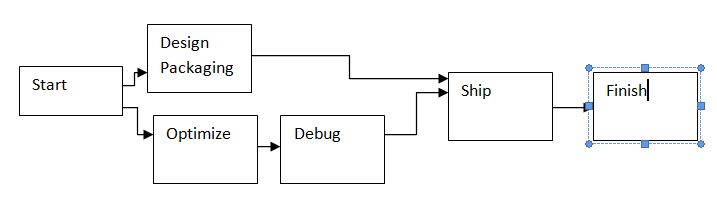
\includegraphics[height=40mm]{pop.png}`
\caption{A Partial ORder Plan}

\end{center}
\end{figure}
\end{enumerate}
\item %Problem 3
\begin{enumerate}
\item %Problem 3a
P(S) = (0.10664)(0.7) + (0.89336)(0.1) = 0.163984 
\item %Problem 3b
$P(\lnot S,C | G) = P(\lnot S | G) P(C | G)$ = (0.3)(0.8) = 0.24\\
$P(\lnot S,C | \lnot G) = P(\lnot S | \lnot G) P(C | \lnot G)$ = (0.9)(0.1) = 0.09 \\

\item %Problem 3c
$P(\lnot S, C, G, D, \lnot W) = P(\lnot S | G)P(C | G)P(G|D,\lnot W)P(D)P(\lnot W) = (0.1)(0.8)(0.8)(0.01)(0.91)=0.0005824$

\item %Problem 3d
$P(G|D) = 0.95*0.09+0.80*0.81 = 0.7335$ \\
$P(G) = 0.01*0.09*0.95+0.01*0.81*0.8+0.99*0.09*0.6+0.99*0.81*0.05 = 0.101$

\item %Problem 3e
$P(S) = P(S|G)P(G)$, and since we computed P(G) in 3(d), we can compute this number.\\
$P(S) = 0.7*0.101+0.1*0.899 = 0.1606$ 

\item %Problem 3f 
$P(D | S) = P(G | S)P(D | G)$ = $\frac{P(S|G)P(G)}{P(S)} \frac{P(G|D)P(D)}{P(G)} = 0.440*.0799 = 0.0352$ 
\end{enumerate}

\item %problem 4
\begin{enumerate}
\item 
\begin{tabular}{|c|c|c|}
\hline
Variable Eliminiated & Factors Used & Factor Generated \\
\hline
A & $f_{1}(A), f_{2}(A,B,C)$ & $f_{3}(B,C)$ \\ 
B & $f_{4}(B), f_{3}(B,C), f_{5}(B,D)$ & $f_{6}(C,D)$ \\
C & $f_{6}(C,D), f_{7}(C,E)$ & $f_{8}(D,E)$ \\
D & $f_{8}(D,E), f_{9}(D,F)$ & $f_{10}(E,F)$ \\
E & $f_{10}(E,F), f_{11}(E,G)$ & $f_{12}(F,G)$ \\  
F & $f_{12}(F,G)$ & $f_{13}(G)$ \\
\hline
\end{tabular}
\item 
This question has me a little confused. I think it is looking for an elimination ordering which is exponential in runtime. I think that if you start eliminating nodes in the reverse order as what was done for part a, more nodes then just two will be created per elimination, but I'm not quite sure how to put that into a table. 
\end{enumerate}

\item % Problem 5

\begin{enumerate}
\item %5a
We can compute the prior probabailities of $X_{1}$ and $X_{2}$.  \\
$P(X_{1}) = 0.8*0.5+0.3*0.5 = 0.55$ \\
$P(X_{2}) = 0.5*0.5+0.1*0.5 = 0.30$

Knowing this, we can compute$ P(Y|X_{1})=\frac{0.8*0.5}{0.55}= 0.72$  and \\
$ P(Y|\lnot X_{1})=\frac{0.2*0.5}{0.45}= 0.222$ using bayes rule. 

If $X_{1}=T$ then the predicted class label is Y=T and if $X_{1}=F$ then the predicted class label is Y=F

The predicted error is then 0.28 * 0.55 + 0.22 * 0.45 = 0.253

If instead we use $X_{2}$
$ P(Y|X_{2})=\frac{0.5*0.5}{0.30}= 0.83$  and \\
$ P(Y|\lnot X_{2})=\frac{0.5*0.5}{0.70}= 0.357$.

The predicted error is then 0.17* 0.5 + 0.357* 0.5 =  0.2635
\item %5b
If we use both attributes then the error rate equals \\
$P(T,T | Y=F) + P(T,F|Y=F) + P(F,T|Y=F) + P(F,F|Y=T) = \\
(0.3)(0.1)+(0.3)(0.9)+(0.7)(0.1)+(0.2)(0.5) = 0.47$
\item %5c

\end{enumerate}


\item % Problem 6
\begin{enumerate}
\item 
P(A=0|y=T) = 0.25, P(B=0|y=T) = 0.5, P(C=1|y=T) = 0.5 \\
P(A=0|y=F) = 0.66, P(B=0|y=F) = 0.33 P(C=1|y=F) = 0.33 \\
P(Y=T)P(A=0|y=T)P(B=0|y=T) P(C=1|y=T)=0.571*0.25*0.5*0.5 = 0.0356875 \\
P(Y=F)P(A=0|y=F)P(B=0|y=F) P(C=1|y=F)=0.428*0.66*0.33*0.33 = 0.0307 \\

Therefor a naive bayes classifier would classify this example as y=T. 
\item 
The main weakness of naive Bayesian classifiers is that they assume independence amongst the input variables. The only way the other classifiers can improve upon the results generated by the naive bayes algorithm is by utilizing some depenedence relation between the input variables. If the variables are known to be independent random variables, then no algorithm can improve upon the Naive bayes classifier. 

\end{enumerate}
\item % Problem 7
Since we know $W_{j} \leftarrow W_{j} + \alpha \times Err \times g'(in) \times x_{j}$, and $f(x) = \frac{1}{2b}(xw+b)$ This means that $f'(x) = \frac{1}{2b}w$. \\
Therefore the weight adjustment rule equals
\[W_{j} \leftarrow W_{j} + \alpha \times \epsilon \times \frac{1}{2b}W_{j}\times x_{j}\]
\end{enumerate}



\end{document}
